Thus far in this work a solution to simplify and automate design the process of all digital PLL loop filter designs comprised of (1) an automated loop filter optimization and design engine, and (2) a discrete-event, time domain PLL simulator to evaluate the designed filters with full time-discretization and quantization nonlinearity effects. Now, in this discussion, the performance of the presented design solution will first be evaluated with a design example. Then, a comparison of the presented solution then will be made to existing solutions in literature, pointing out advantages and disadvantages will be made. Finally, a general discussion will be made covering areas of improvement, reasoning for the central design choices made, and considerations for usage the framework.

\subsection{Design exercise using this work}
The design of a loop filter for the PLL with the system level specifications of table \ref{design_specs} will be considered here, with the intent of optimizing phase noise. These specifications, where the TDC resolution in steps equals the divider ratio, is equivalent to a special case of a TDC-less PLL where a 150-step synchronous counter is used as a divider, and the loop filter directly samples the state of the synchronous counter. For filter design, a PI-controller loop filter prototype was utilized in the optimizer.

% \scriptsize
\begin{table}[h!]
	\centering
	\def\arraystretch{1.5}		
	\setlength\arrayrulewidth{0.75pt}
	\setlength{\tabcolsep}{1em} % for the horizontal padding
	\begin{tabular}{|l|r|l|}
		\hline 
		\rule[-1ex]{0pt}{2.5ex} \cellcolor{gray!40}\textbf{Parameter} & \cellcolor{gray!40}\textbf{Value} & \cellcolor{gray!40}\textbf{Unit }\\ 
		\hline 
		\rule[-1ex]{0pt}{2.5ex} \textbf{Output Frequency}  & 2.4 & GHz \\ 
		\hline 
		\rule[-1ex]{0pt}{2.5ex} \textbf{Ref. frequency} & 16 & MHz\\ 
		\hline 
		\rule[-1ex]{0pt}{2.5ex} \textbf{Divider ratio} & 150  &\\ 
		\hline 
		\rule[-1ex]{0pt}{2.5ex} \textbf{TDC resolution} & 150  & steps/reference cycle\\ 
		\hline 
		\rule[-1ex]{0pt}{2.5ex} \textbf{DCO gain $K_{DCO}$} & $10^4$ & Hz/LSB \\ 
		\hline 
		\rule[-1ex]{0pt}{2.5ex} \textbf{DCO Phase noise} & -80 & dBc/Hz at $\Delta f=10^6$ Hz \\ 
		\hline 
		\rule[-1ex]{0pt}{2.5ex} \textbf{Lock Time} & $\leq$ 25 & $\mu$s \\ 
		\hline 
		\rule[-1ex]{0pt}{2.5ex} \textbf{Lock $\Delta f$ tolerance} & $10^5$ & Hz \\ 
		\hline 
		\rule[-1ex]{0pt}{2.5ex} \textbf{Digital filter word resolution} & $\leq$ 16 & bits \\ 
		\hline 
		\rule[-1ex]{0pt}{2.5ex} \textbf{Residual phase modulation} & minimize &  \\ 
		\hline 
	\end{tabular} 
	% \caption{Assigned specifications for branch line hybrid design.}
	% \label{asgn_specs}
	\caption{System-level specifications}
	\label{design_specs}
\end{table}   

\subsubsection{Result of filter optimization.}
Table \ref{filter_params} contains the optimized filter parameters obtained from the filter design optimizer developed in this work. $\{K$, $K_i$, $K_p$, $f_z\}$ are the continuous model parameters of section \ref{cont_pi_filt_des}, and $\{a_0$, $a_1$, $a_2$, $b_0$, $b_1\}$ are the filter coefficients for the discrete-time direct form-I filter structure of section \ref{disc_lf_comp_pi}. The estimated bandwidth for the filter is 144.8 kHz, and the lock time is estimated to be 19.3 $\mu$s. Table \ref{dig_filter_params} contains the digitized version of the discrete time filter, based on a selection for word size determined via optimization for finite word effects. The final data words are 13 bits in length.  
% \scriptsize
\begin{table}[h!]
	\centering
	\def\arraystretch{1.5}		
	\setlength\arrayrulewidth{0.75pt}
	\setlength{\tabcolsep}{1em} % for the horizontal padding
	\begin{tabular}{|l|r|l|}
		\hline 
		\rule[-1ex]{0pt}{2.5ex} \cellcolor{gray!40}\textbf{Parameter} & \cellcolor{gray!40}\textbf{Value} & \cellcolor{gray!40}\textbf{Unit }\\ 
		\hline 
		\rule[-1ex]{0pt}{2.5ex} \textbf{$K$}  & $1.343792\times10^{11}$ &  \\ 
		\hline 
		\rule[-1ex]{0pt}{2.5ex} \textbf{$K_i$}  & $1.343792\times10^{7}$ &  \\ 
		\hline 
		\rule[-1ex]{0pt}{2.5ex} \textbf{$K_p$}  & $7.331074\times10^{1}$ &  \\ 
		\hline 
		\rule[-1ex]{0pt}{2.5ex} \textbf{$f_z$} & $2.917324\times10^4$ & Hz\\ 
		\hline 
		\rule[-1ex]{0pt}{2.5ex} \textbf{$b_0$}  & $7.4150613906\times10^1$  &\\ 
		\hline 
		\rule[-1ex]{0pt}{2.5ex} \textbf{$b_1$}  & $-7.3310743796\times10^1$  & \\ 
		\hline 
		\rule[-1ex]{0pt}{2.5ex} \textbf{$a_0$}  & $1.0\times10^0$  &\\ 
		\hline 
		\rule[-1ex]{0pt}{2.5ex} \textbf{$a_1$}  & $-1.0\times10^0$  & \\ 
		\hline 
		\rule[-1ex]{0pt}{2.5ex} \textbf{$a_2$}  & $0.0\times10^0$  & \\ 
		\hline 
		\rule[-1ex]{0pt}{2.5ex} Estimated bandwidth & $1.448234\times10^5$ & Hz \\ 
		\hline 
		\rule[-1ex]{0pt}{2.5ex} Estimated lock time & $1.934253\times10^{-5}$ & seconds \\ 
		\hline 
	\end{tabular} 
	% \caption{Assigned specifications for branch line hybrid design.}
	% \label{asgn_specs}
	\caption{PLL parameters determined from filter design and optimization process.}
	\label{filter_params}
\end{table}   

\begin{table}[h!]
	\centering
	\def\arraystretch{1.5}		
	\setlength\arrayrulewidth{0.75pt}
	\setlength{\tabcolsep}{1em} % for the horizontal padding
	\begin{tabular}{|l|r|r|l|}
		\hline 
		\rule[-1ex]{0pt}{2.5ex} \cellcolor{gray!40}\textbf{Parameter} & \cellcolor{gray!40}\textbf{Value} & \cellcolor{gray!40}\textbf{Value (digital) } & \cellcolor{gray!40}\textbf{Value Error}\\ 
		\hline 
		\rule[-1ex]{0pt}{2.5ex} Total dataword bits  & 13 & & \\ 
		\hline 
		\rule[-1ex]{0pt}{2.5ex} Sign bits  & 1 & & \\ 
		\hline 
		\rule[-1ex]{0pt}{2.5ex} Integer bits & 7 & & \\ 
		\hline 
		\rule[-1ex]{0pt}{2.5ex} Fractional bits  & 5 & & \\ 
		\hline 
		\rule[-1ex]{0pt}{2.5ex} \textbf{$b_0$} & $7.415625\times10^1$ & \texttt{0b0100101000101}  & $+5.636094\times10^{-3}$\\ 
		\hline 
		\rule[-1ex]{0pt}{2.5ex} \textbf{$b_1$}  & $-7.331250\times10^1$ & \texttt{0b1111011010110}  & $-1.756204\times10^{-3}$\\ 
		\hline 
		\rule[-1ex]{0pt}{2.5ex} \textbf{$a_0$}  & $1.0\times10^0$ & \texttt{0b0000000100000} & $0.0\times10^0$ \\ 
		\hline 
		\rule[-1ex]{0pt}{2.5ex} \textbf{$a_1$}  & $-1.0\times10^0$ & \texttt{0b1111111100000} & $0.0\times10^0$ \\ 
		\hline 
		\rule[-1ex]{0pt}{2.5ex} \textbf{$a_2$}  & $0.0\times10^0$ & \texttt{0b0000000000000} & $0.0\times10^0$ \\ 
		\hline 
	\end{tabular} 
	% \caption{Assigned specifications for branch line hybrid design.}
	% \label{asgn_specs}
	\caption{Loop filter parameters after digitization and optimization for data word length.}
	\label{dig_filter_params}
\end{table}  

\subsubsection{Result of transient and phase noise simulation.}
The simulation engine implemented in this work was utilized to run a time domain simulation to verify the designed filter. Figures \ref{fig:trans_lf} and \ref{fig:trans_inst_freq} demonstrate the transient response of the PLL with an initial frequency error of 12 MHz (0.5\% of final frequency). It is observed that the PLL design stably approaches the target frequency in approximately 23 $\mu$s. Figures \ref{fig:trans_det} illustrate the BBPD and TDC outputs during this inital transient. It is observed that the TDC output gives the dominant feedback, unit it reaches an output word of 0, where the BBPD then begins providing feedback in the steady state condition of the PLL. Figure \ref{fig:trans_phase_noise} is the result of a phase noise calculation for the simulated PLL in an interval beginning immediately after detection of lock. The spectrum closely approximates that designed for, with some small additional peaking.
	\begin{figure}[htb!]
	    \centering
	    \begin{subfigure}{0.5\textwidth}
	        \centering
	        \center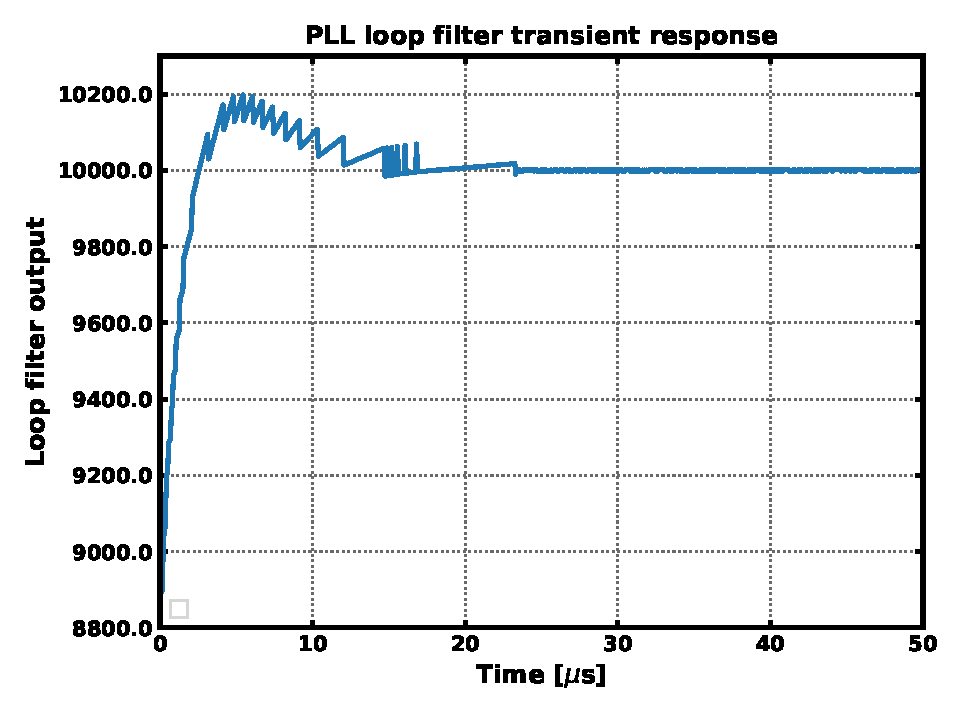
\includegraphics[width=1.0\textwidth, angle=0]{figs/trans_loop_filter.pdf}
	        \caption{ }
	        \label{fig:trans_lf}
	    \end{subfigure}%
	    \begin{subfigure}{0.5\textwidth}
	        \centering
	        \center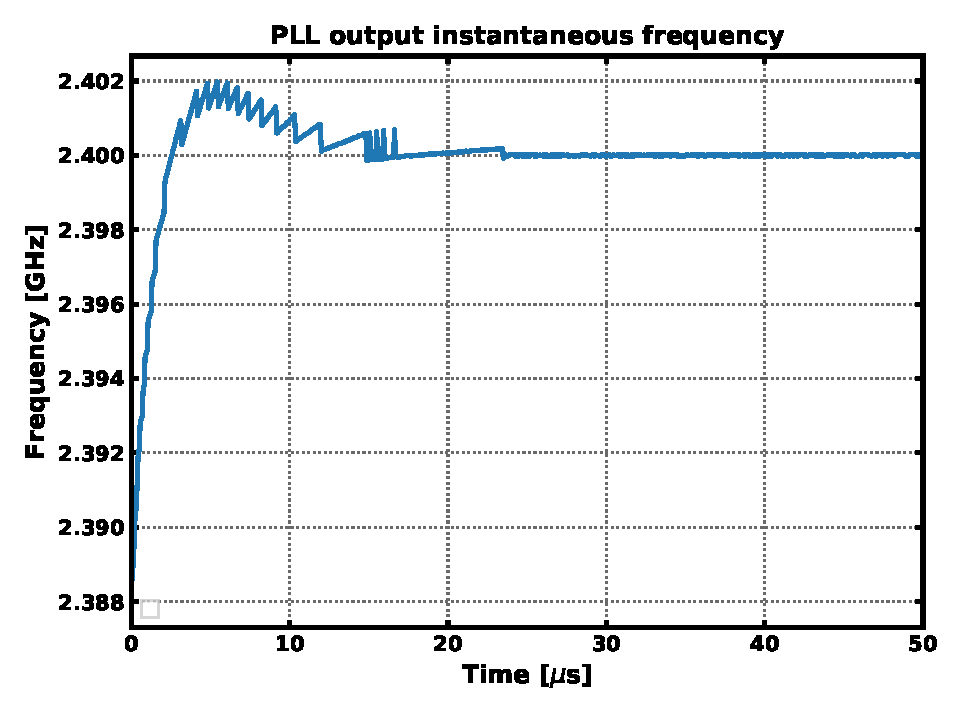
\includegraphics[width=1.0\textwidth, angle=0]{figs/trans_inst_freq.pdf}
	        \caption{ }
	        \label{fig:trans_inst_freq}
	    \end{subfigure}
	    % \caption{Approximate model for ring oscillator inverter delay cell.}
	    \label{fig:trans_sim1}
	    \caption{Simulation with 0.5\% initial frequency error: \textbf{(a)} Loop filter transient response, \textbf{(b)} PLL output instantaneous frequency.}
	\end{figure}

	\begin{figure}[htb!]
	    \centering
	    \begin{subfigure}{0.5\textwidth}
	        \centering
	        \center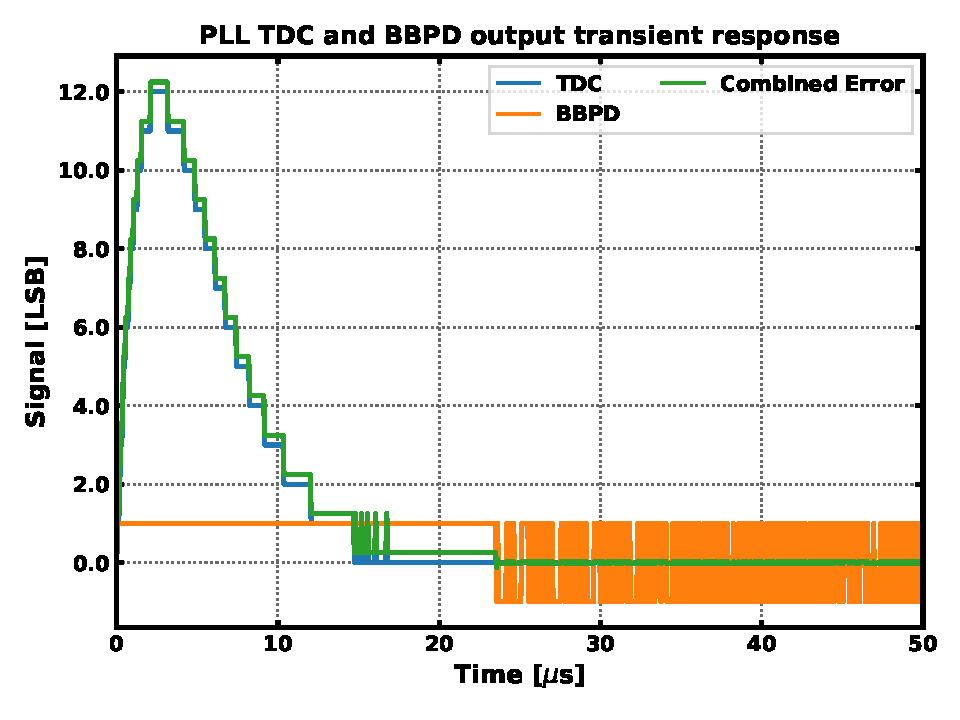
\includegraphics[width=1.0\textwidth, angle=0]{figs/trans_tdc_bbpd.pdf}
	        \caption{ }
	        \label{fig:trans_det}
	    \end{subfigure}%
	    \begin{subfigure}{0.5\textwidth}
	        \centering
	        \center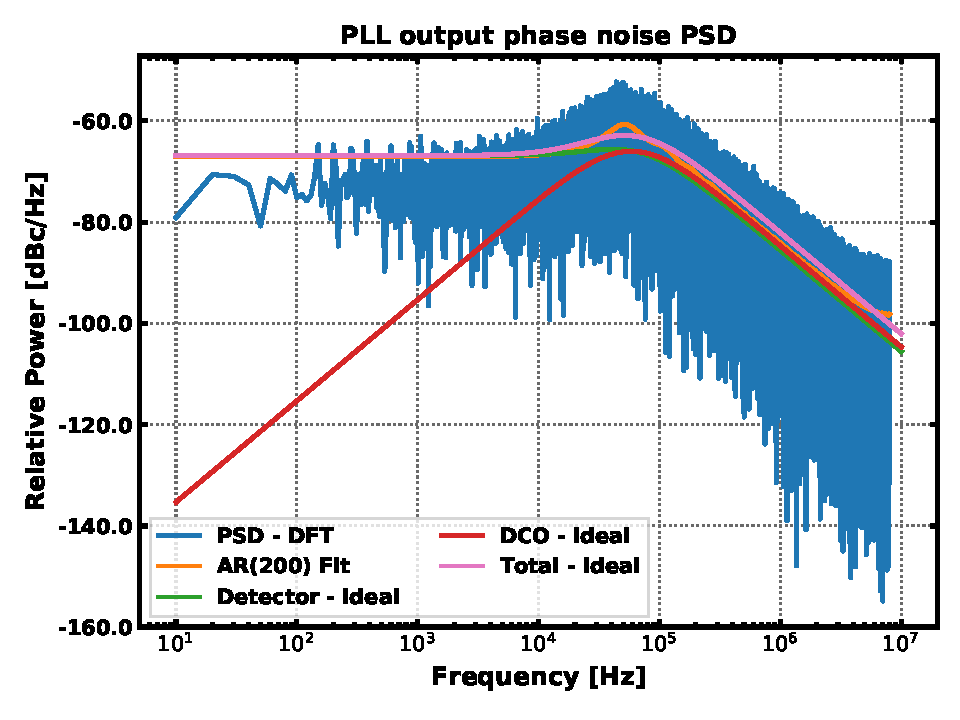
\includegraphics[width=1.0\textwidth, angle=0]{figs/trans_phase_noise.pdf}
	        \caption{ }
	        \label{fig:trans_phase_noise}
	    \end{subfigure}
	    % \caption{Approximate model for ring oscillator inverter delay cell.}
	    \label{fig:trans_sim2}
	    \caption{Simulation with 12 MHz (0.5\%) initial frequency error: \textbf{(a)} BBPD/TDC detector responses, \textbf{(b)} PLL output phase noise power spectrum.}
	\end{figure}

\subsubsection{Result of parametric sweep and variation analysis.}
The Monte-Carlo sampling and parametric sweep facilities in the simulator designed in this work were used to run analysis for effects of variation of DCO gain $K_{DCO}$ and initial frequency error of the PLL. Figure \ref{fig:sweep_kdco} shows a parametric sweep of $K_{DCO}$, with lock time being measured. It is observed that the lock time is nearly flat in the range 7300-18000 Hz/LSB, meaning that there is a tolerance of -2700/+8000 Hz LSB for KDCO about the nominal 10000 Hz/LSB specified. This specification can be utilized in the design of a physical DCO to constrain maximum acceptable variation across PVT. Figure \ref{fig:sweep_finit} demonstrates the simulated effect of initial frequency error on lock time. It is seen that PLL stably locks to the target frequency within the entire simulated interval of $\pm$ 60 MHz from 2.4GHz, implying that the capture range of the PLL is $>120$ MHz. This specification can be translated into a requirement for initial coarse frequency calibration needed before starting the PLL. Figures \ref{fig:mc_trans} and \ref{fig:mc_hist} are the results of a variation analysis simulation utilizing the Monte-Carlo sampling engine implemented in this work. The simulation was configured to vary $K_{DCO}$ with a standard deviation of 20 \% of the nominal value, and to vary the inital starting frequency with a standard deviation of 60 MHz (0.025 \% of the final frequency). The simulation sample size is 1000. The transient responses from the simulation figure \ref{fig:mc_trans} are all stable, and figure \ref{fig:mc_hist} shows the histogram for measured lock time subject to the described variation. The mean lock time was 24.57 $\mu$s, meeting the 25 $\mu$s lock time set for the PLL, and the upper bound for a 99\% confidence interval on the data is 50.75 $\mu$s. A set of extracted parameters from these simulations are in table \ref{simulation_params}. The Monte-Carlo simulations presented here are useful to analyze the range of variation in which the designed PLL can tolerate, as well as determine the expected performance varation, so well informed decisions on a PLL design can be made before moving into transistor level implementation and simulation. 

	\begin{figure}[htb!]
	    \centering
	    \begin{subfigure}{0.5\textwidth}
	        \centering
	        \center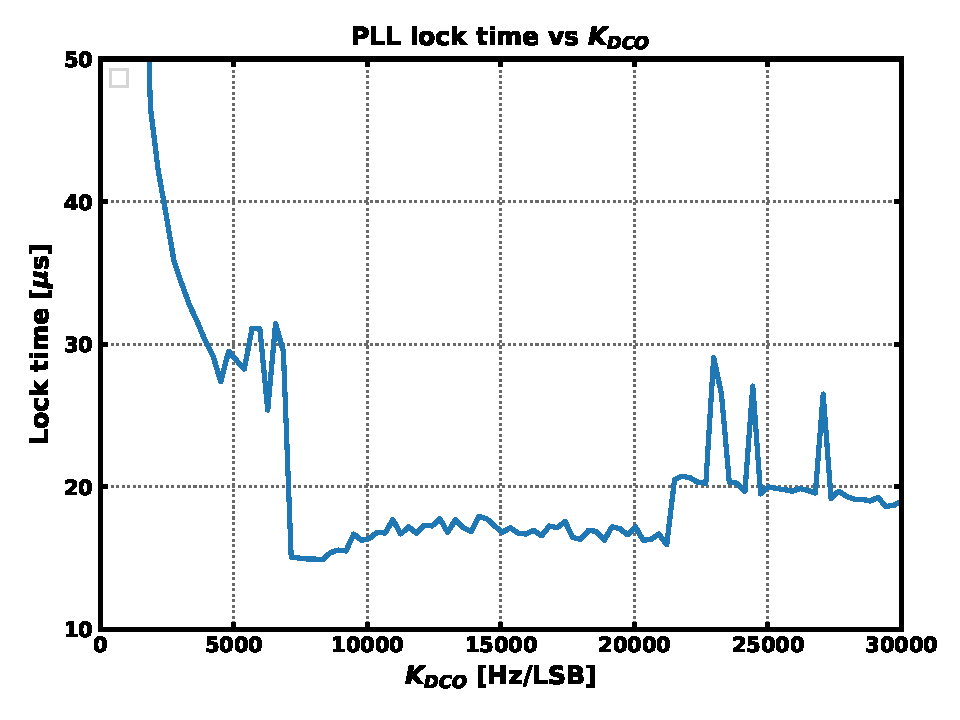
\includegraphics[width=1.0\textwidth, angle=0]{figs/_kdco_sweep.pdf}
	        \caption{ }
	        \label{fig:sweep_kdco}
	    \end{subfigure}%
	    \begin{subfigure}{0.5\textwidth}
	        \centering
	        \center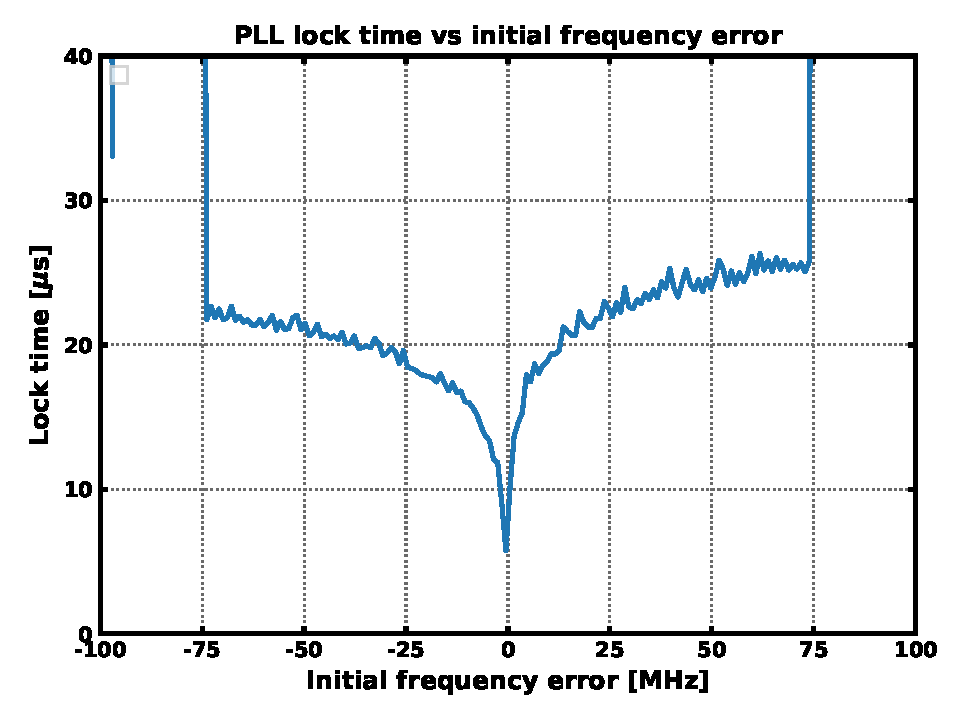
\includegraphics[width=1.0\textwidth, angle=0]{figs/_finit_sweep.pdf}
	        \caption{ }
	        \label{fig:sweep_finit}
	    \end{subfigure}
	    % \caption{Approximate model for ring oscillator inverter delay cell.}
	    \label{fig:sweep_sim}
	    \caption{\textbf{(a)} PLL lock time simulation with KDCO swept, 12 MHz (0.5\%) initial frequency error, \textbf{(b)} PLL lock time simulation with initial frequency error swept.}
	\end{figure}

	\begin{figure}[htb!]
	    \centering
	    \begin{subfigure}{0.5\textwidth}
	        \centering
	        \center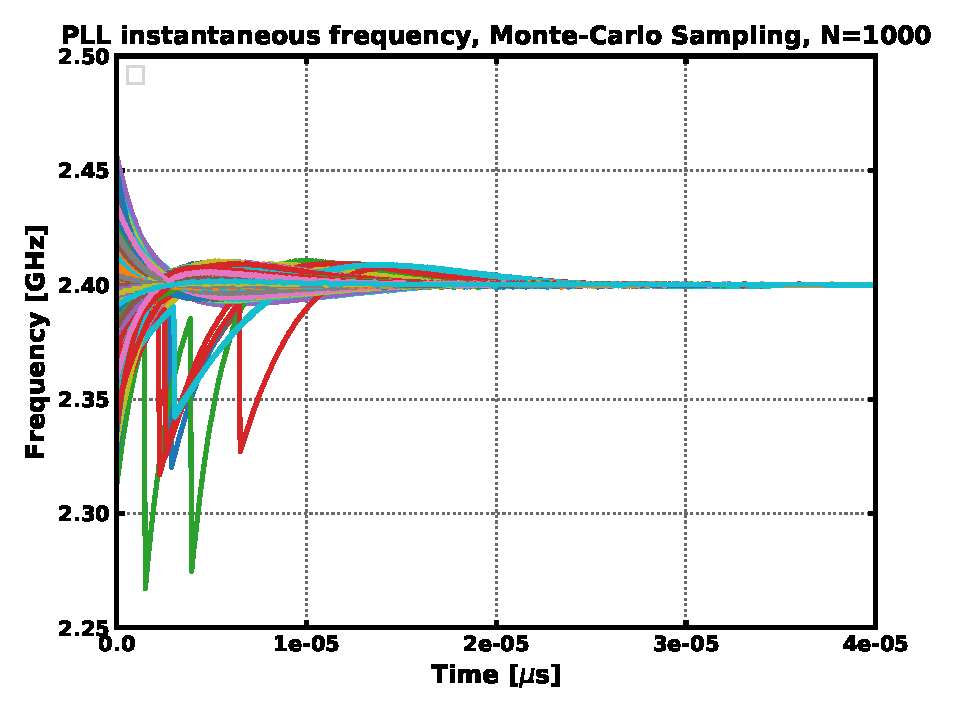
\includegraphics[width=1.0\textwidth, angle=0]{figs/mc_trans.pdf}
	        \caption{ }
	        \label{fig:mc_trans}
	    \end{subfigure}%
	    \begin{subfigure}{0.5\textwidth}
	        \centering
	        \center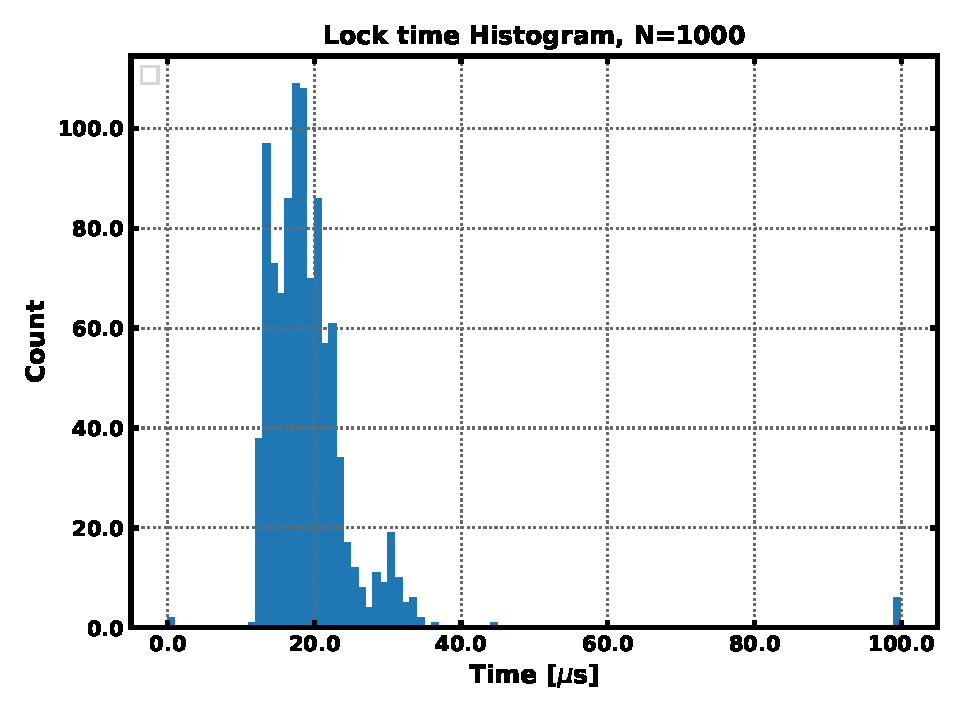
\includegraphics[width=1.0\textwidth, angle=0]{figs/mc_hist.pdf}
	        \caption{ }
	        \label{fig:mc_hist}
	    \end{subfigure}
	    % \caption{Approximate model for ring oscillator inverter delay cell.}
	    \label{fig:mc_sim}
	    \caption{Monte-Carlo simulation with 1000 samples, 20\% RMS deviation in KDCO, and 60 MHz (2.5\%) RMS deviation in initial frequency error \textbf{(a)} Frequency transient responses, \textbf{(b)} Lock time histogram.}
	\end{figure}

\begin{table}[h!]
	\centering
	\def\arraystretch{1.5}		
	\setlength\arrayrulewidth{0.75pt}
	\setlength{\tabcolsep}{1em} % for the horizontal padding
	\begin{tabular}{|l|r|l|}
		\hline 
		\rule[-1ex]{0pt}{2.5ex} \cellcolor{gray!40}\textbf{Parameter} & \cellcolor{gray!40}\textbf{Value} & \cellcolor{gray!40}\textbf{Unit }\\ 
		\hline 
		\rule[-1ex]{0pt}{2.5ex} \textbf{$K_{DCO}$ Tolerance}  & -2700/+8000 & MHz/LSB \\ 
		\hline 
		\rule[-1ex]{0pt}{2.5ex} \textbf{Capture range}  & $>$ 120 & MHz \\ 
		\hline 
		\rule[-1ex]{0pt}{2.5ex} \textbf{Mean lock time}  & 24.57263 & $\mu$s \\ 
		\hline 
		\rule[-1ex]{0pt}{2.5ex} \textbf{Lock time $\sigma$} & 8.286061 & $\mu$s\\ 
		\hline 
		\rule[-1ex]{0pt}{2.5ex} \textbf{Lock time 99 \% CI upper bound} & 50.75  & $\mu$s\\ 
		\hline 
	\end{tabular} 
	% \caption{Assigned specifications for branch line hybrid design.}
	% \label{asgn_specs}
	\caption{PLL parameters extracted from variance and parameter sweep simulations.}
	\label{simulation_params}
\end{table}

\subsubsection{Design method 2}
\hl{make sure captions and labels are unique}
	\begin{figure}[htb!]
	    \centering
	    \begin{subfigure}{0.5\textwidth}
	        \centering
	        \center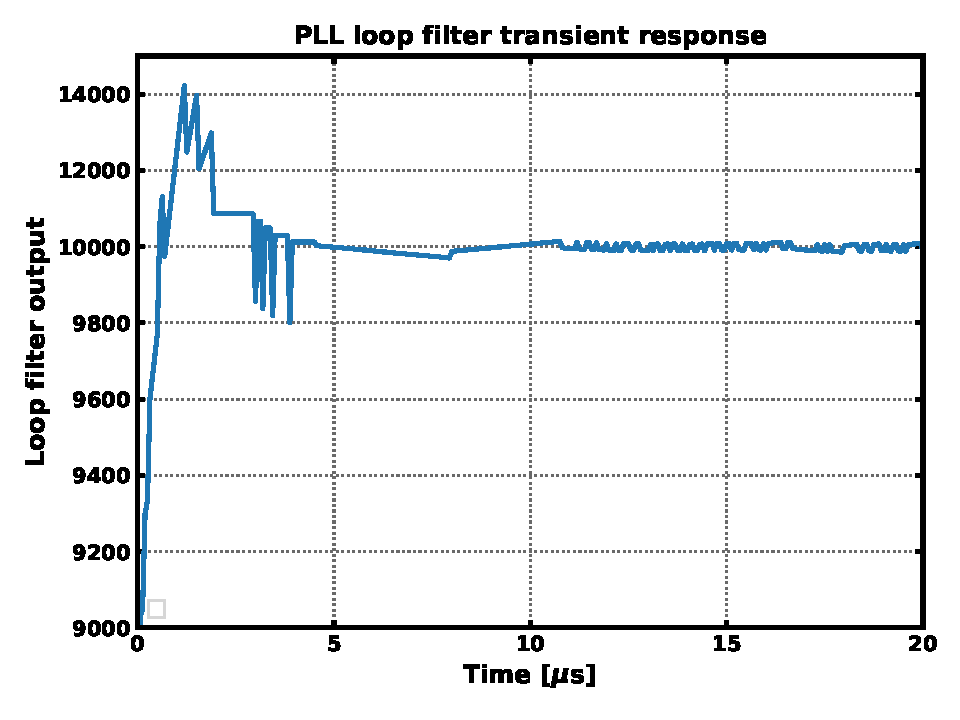
\includegraphics[width=1.0\textwidth, angle=0]{figs/trans_loop_filter_fast.pdf}
	        \caption{ }
	        \label{fig:trans_lf_fast}
	    \end{subfigure}%
	    \begin{subfigure}{0.5\textwidth}
	        \centering
	        \center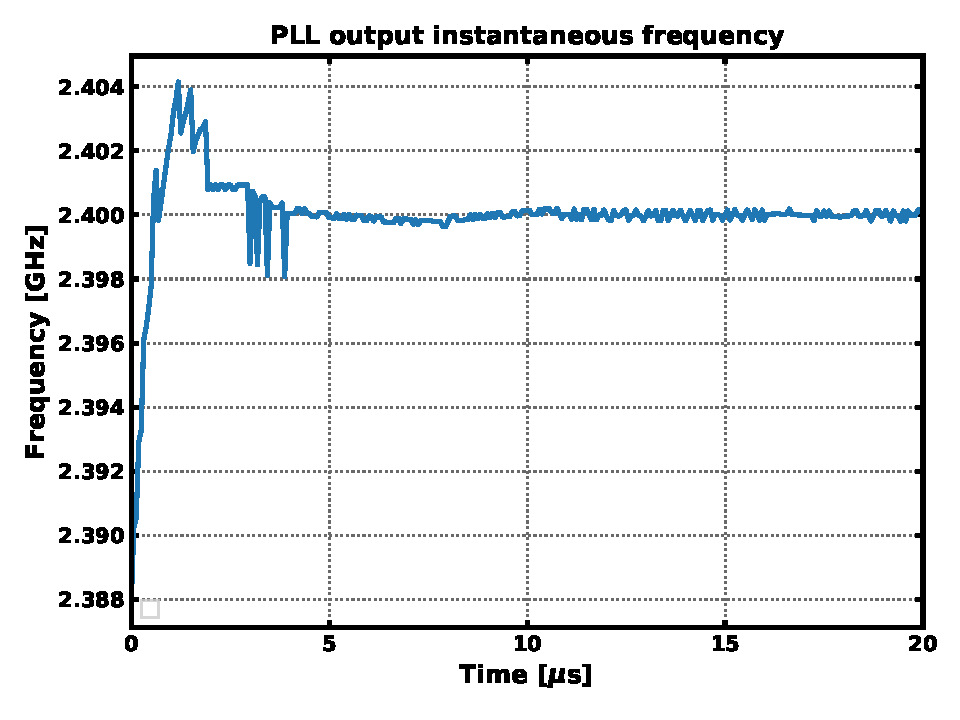
\includegraphics[width=1.0\textwidth, angle=0]{figs/trans_inst_freq_fast.pdf}
	        \caption{ }
	        \label{fig:trans_inst_freq_fast}
	    \end{subfigure}
	    % \caption{Approximate model for ring oscillator inverter delay cell.}
	    \label{fig:trans_sim1_fast}
	    \caption{Simulation with 0.5\% initial frequency error: \textbf{(a)} Loop filter transient response, \textbf{(b)} PLL output instantaneous frequency.}
	\end{figure}

	\begin{figure}[htb!]
	    \centering
	    \begin{subfigure}{0.5\textwidth}
	        \centering
	        \center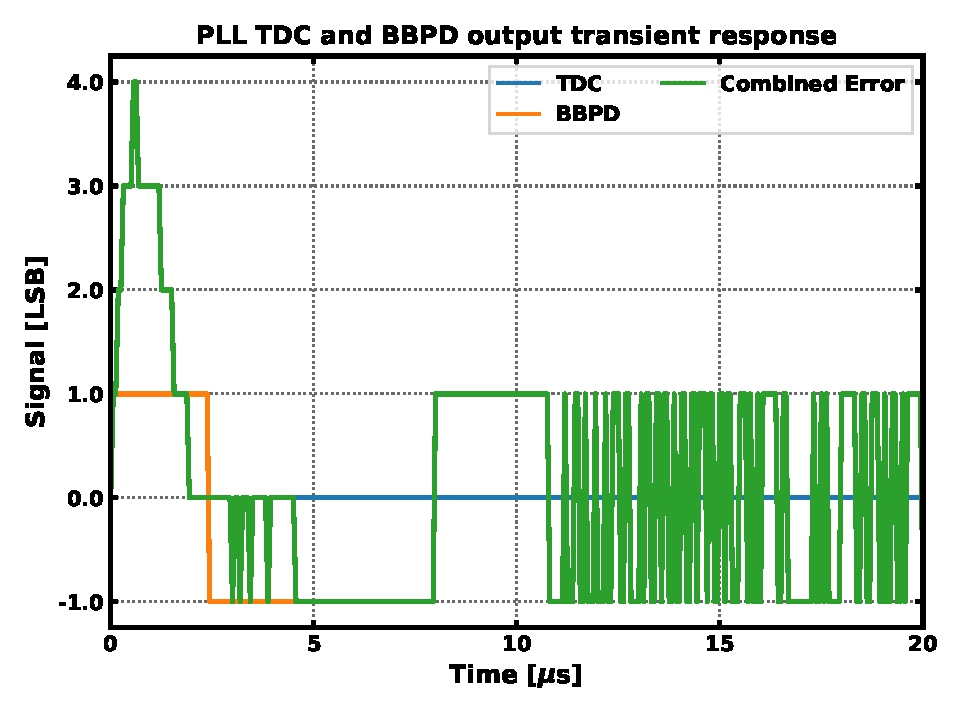
\includegraphics[width=1.0\textwidth, angle=0]{figs/trans_tdc_bbpd_fast.pdf}
	        \caption{ }
	        \label{fig:trans_det_fast}
	    \end{subfigure}%
	    \begin{subfigure}{0.5\textwidth}
	        \centering
	        \center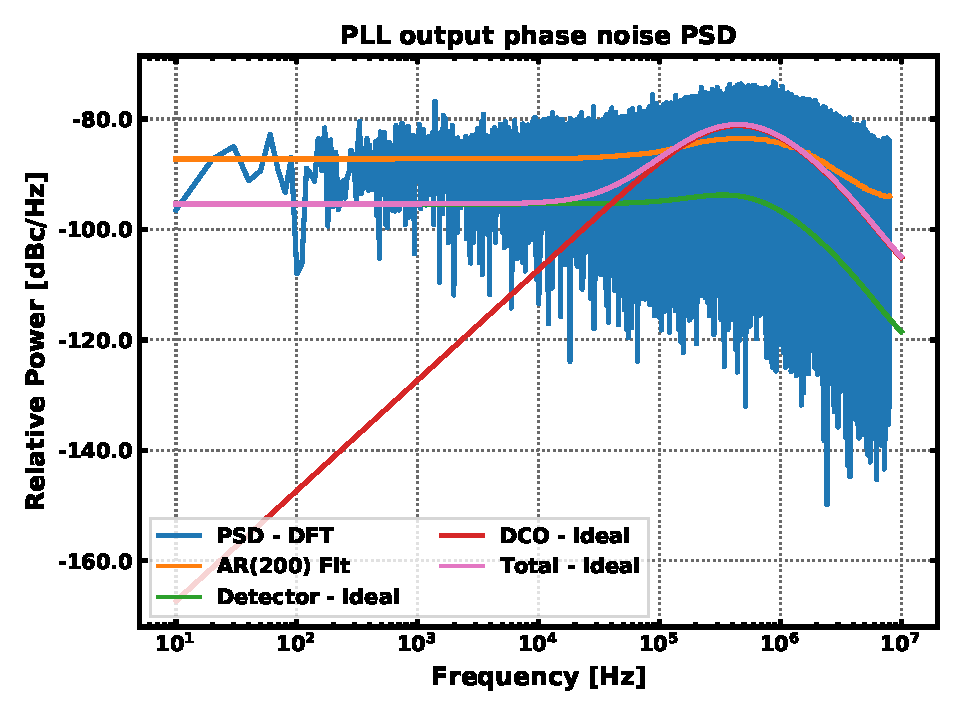
\includegraphics[width=1.0\textwidth, angle=0]{figs/trans_phase_noise_fast.pdf}
	        \caption{ }
	        \label{fig:trans_phase_noise_fast}
	    \end{subfigure}
	    % \caption{Approximate model for ring oscillator inverter delay cell.}
	    \label{fig:trans_sim2_fast}
	    \caption{Simulation with 12 MHz (0.5\%) initial frequency error: \textbf{(a)} BBPD/TDC detector responses, \textbf{(b)} PLL output phase noise power spectrum.}
	\end{figure}

	\begin{figure}[htb!]
	    \centering
	    \begin{subfigure}{0.5\textwidth}
	        \centering
	        \center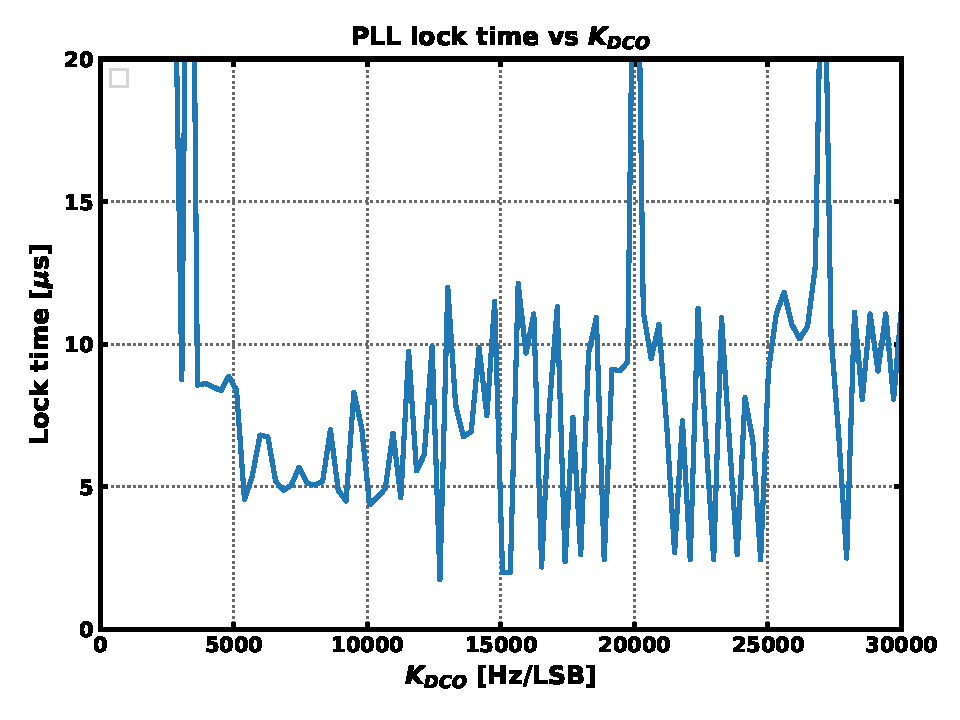
\includegraphics[width=1.0\textwidth, angle=0]{figs/_kdco_sweep_fast.pdf}
	        \caption{ }
	        \label{fig:sweep_kdco}
	    \end{subfigure}%
	    \begin{subfigure}{0.5\textwidth}
	        \centering
	        \center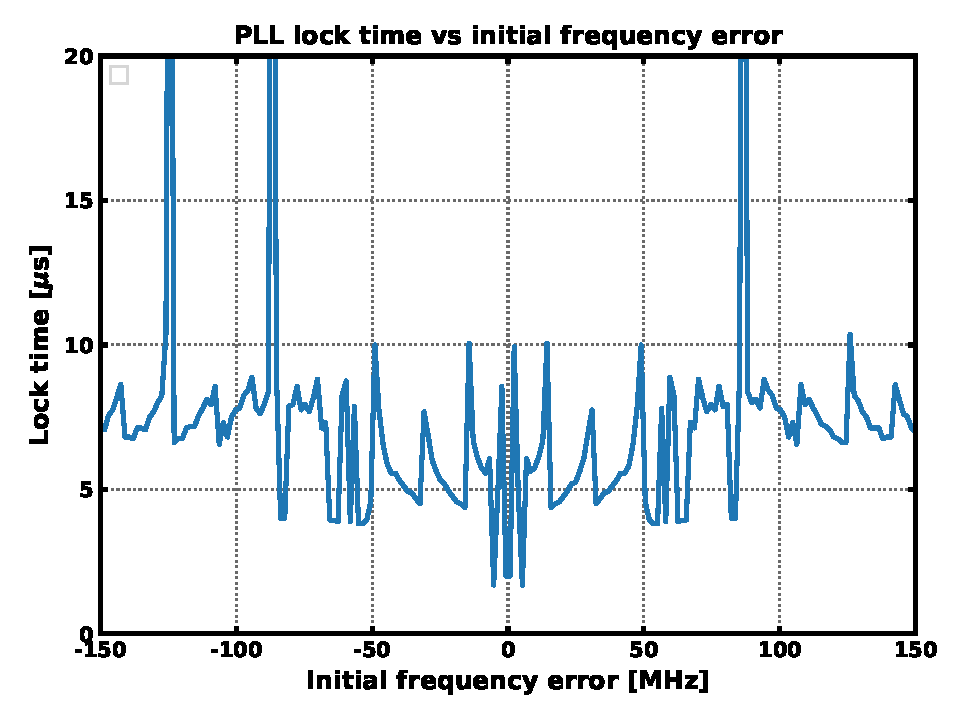
\includegraphics[width=1.0\textwidth, angle=0]{figs/finit_sweep_fast.pdf}
	        \caption{ }
	        \label{fig:sweep_finit}
	    \end{subfigure}
	    % \caption{Approximate model for ring oscillator inverter delay cell.}
	    \label{fig:sweep_sim}
	    \caption{\textbf{(a)} PLL lock time simulation with KDCO swept, 12 MHz (0.5\%) initial frequency error, \textbf{(b)} PLL lock time simulation with initial frequency error swept.}
	\end{figure}

	\begin{figure}[htb!]
	    \centering
	    \begin{subfigure}{0.5\textwidth}
	        \centering
	        \center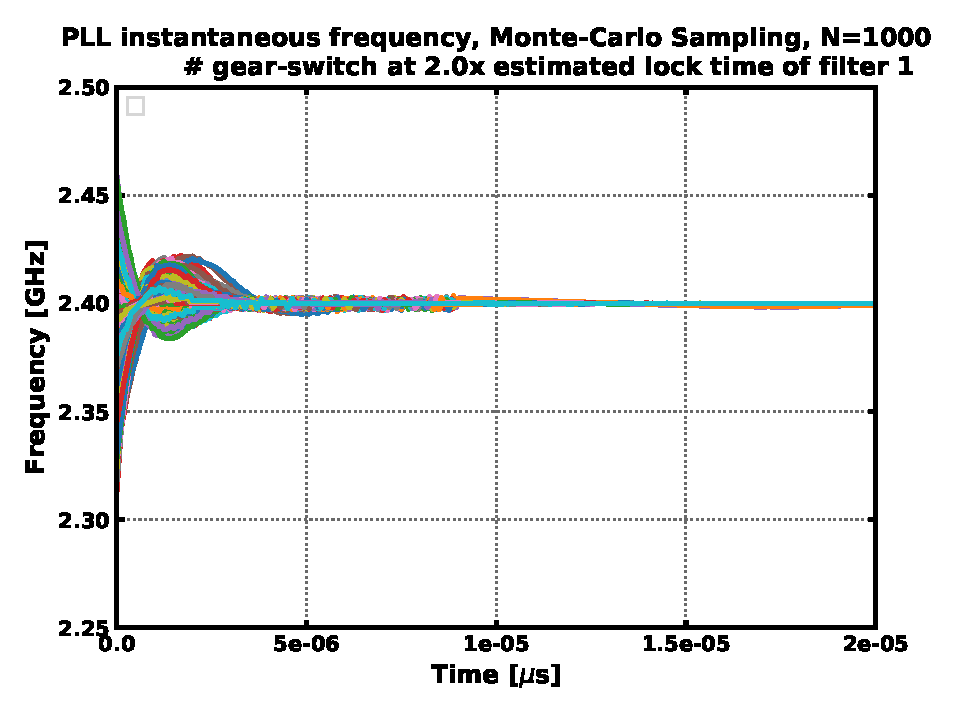
\includegraphics[width=1.0\textwidth, angle=0]{figs/mc_trans_2x.pdf}
	        \caption{ }
	        \label{fig:mc_trans}
	    \end{subfigure}%
	    \begin{subfigure}{0.5\textwidth}
	        \centering
	        \center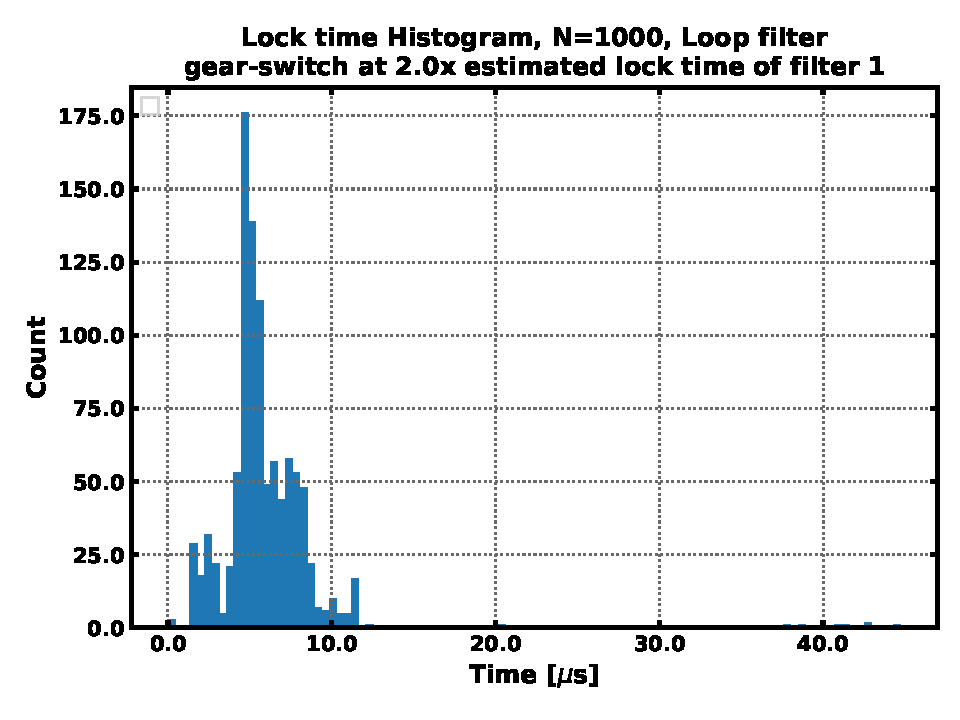
\includegraphics[width=1.0\textwidth, angle=0]{figs/mc_hist_fast_2x.pdf}
	        \caption{ }
	        \label{fig:mc_hist}
	    \end{subfigure}
	    % \caption{Approximate model for ring oscillator inverter delay cell.}
	    \label{fig:mc_sim}
	    \caption{Monte-Carlo simulation with 1000 samples, 20\% RMS deviation in KDCO, and 60 MHz (2.5\%) RMS deviation in initial frequency error \textbf{(a)} Frequency transient responses, \textbf{(b)} Lock time histogram.}
	\end{figure}



	% \begin{figure}[htb!]
	% 	\center\includegraphics[width=1.0\textwidth, angle=0]{figs/x.pdf}
	% 	\caption{Transient simulation of optimal design.}
	% 	\label{fig:des_ex_trans}
	% \end{figure}
	% \FloatBarrier

	% \begin{figure}[htb!]
	% 	\center\includegraphics[width=1.0\textwidth, angle=0]{figs/x.pdf}
	% 	\caption{Variation Simulation for KDCO.}
	% 	\label{fig:var_lock}
	% \end{figure}
	% \FloatBarrier

	% \begin{figure}[htb!]
	% 	\center\includegraphics[width=1.0\textwidth, angle=0]{figs/x.pdf}
	% 	\caption{Phase noise.}
	% 	\label{fig:Simulated phase noise.}
	% \end{figure}
	% \FloatBarrier

	% stability criteria - Jurys' stability criteria abs(a0) l.t. a2 for second order z-transfer \cite{xiu_li_meiners_padakanti_2004}
	% - Not phase margin based in optimization, can make stable by using stable choice of PI controller (two poles only) - poles should be in unit circle...
\FloatBarrier
\subsection{Comparison to existing solutions}
Due to the relative youth of all digital PLL design, and discontinuity between the continuous theory of analog PLL and digital PLL design, a smaller body of works exist pertaining to the loop filters for exclusively ADPLLs. Of the existing literature, the majority design approaches utilize discrete-time converted PI-controller loop filters with either bang-bang phase detectors \cite{kratyuk_2007}\cite{safwat_ghoneima_ismail_2011}\cite{zanuso_2009}\cite{xu_abidi_2017} or phase-frequency detectors \cite{kumm_klingbeil_zipf_2010}\cite{chau_chen_2009}. This work takes a similar approach to existing works, focusing on a fixed filter architecture to limit the scope of the problem at hand, and also utilizing a bang-bang phase detector in the PLL architecture. This work, however, differs in its approach to filter design, which is through numerical methods to find optimal filter design, whereas the other works largely focus on closed-form mathematical analysis. The usage of numerical methods here allows for full automation of the loop filter design process, removing work for the designer. 

The criteria and motivation for loop design varies across the surveyed works. Of the surveyed works, several \cite{kratyuk_2007}\cite{kumm_klingbeil_zipf_2010}\cite{chau_chen_2009}\cite{safwat_ghoneima_ismail_2011} do not consider optimization for phase noise as this work principal;y does, but rather consider stability/phase margin \cite{kratyuk_2007}\cite{kumm_klingbeil_zipf_2010}\cite{safwat_ghoneima_ismail_2011}, lock time \cite{chau_chen_2009}\cite{safwat_ghoneima_ismail_2011} and even approach simplicity \cite{kumm_klingbeil_zipf_2010}. The methods that consider optimization of phase noise \cite{zanuso_2009}\cite{xu_abidi_2017} both provide a similar model of PLL dynamics based on a linearized model of the bang-bang phase detector. The design methods of the previous two works are presented with closed-form mathematical theory, using closed loop transfer function modeling to estimate phase noise. It is expected that these approaches yield a better optimization than that afforded with this work when using feedback from a bang-bang phase detector, as this work only attempts to reduce the BBPD noise below that expected for the TDC. This work, however, differs from the latter two as the loop filter is designed to utilize both bang-bang phase detector and TDC feedback, not just bang-bang detector feedback. In terms of optimization criteria, this work is unique in that it is solely focused on minimization of total phase noise power subject to constrained lock-time requirements, both of which are of high interest to the PLL designer.

Few of the existing works consider the implementation of the loop filter design into digital hardware, rather just provide continuous valued coefficients for the filter designs. Of those surveyed, only \cite{kumm_klingbeil_zipf_2010} provides an analysis for quantization noise in terms of SFDR out of the filter design, but lacks the connection to output phase noise. This work uniquely considers (a) the impact of quantization of the digitized filter design, in terms of filter accuracy and output phase noise, and (b) attempts to optimize the digital implementation of the filter in terms of number of bits representing the various components of the filter (i.e. filter coefficients, multipliers, adders) for complexity and performance.

A final advantage of this work not observed in the surveyed literature is the integrated PLL simulator with Monte-Carlo sampling which allows for verification of the designed loop filter with accurate modeling of time-discretization and digital quantization effects. This allows for lock time, phase noise and stability to be verified on the design to ensure it meets the designer's requirements before moving onto testing with transistor level implementations and testing.



\subsection{Design choices and areas of improvement}
\hl{still a work in progess...}
Currently the simulation only handles integer-N PLLs. To extend simulation to fractional-N PLLs, a small simulation time steps (much smaller than reference cycle time used in integer-N case) is needed to reduce quantization noise to low enough levels for the fractional divider noise characteristics to not be overpowered \cite{perrott_2002_sim}. This may prove a limitation in the current simulator, which runs on the order of 60s for the integer-N PLL phase noise simulations.



\begin{itemize}
	\item Discuss choices made in simulator

	\item show effects of non-linearity : simulate PLL without BB-PD (far from ideal)

	\item Low resolution: feedback stops when within 1 LSB in phase lock, response time = t=(n/(m*df)), Use bbpd to add extra resolution.

	\begin{itemize}
		\item Deficiencies, advantages, why they were made
		\item Phase noise/lock time analysis
		\item Analysis - monte-carlo variation to analyze stability/lock time
		\item purpose: to validate filter design
	\end{itemize}
	\item Filter structure choice - PI with added pole. Why is this best (low complexity, no phase error)
	\item Why only phase random walk in oscillator phase noise
	\item Why direct type I implementation
	\item Discuss choices made in loop filter designer/optimizer
	\begin{itemize}
		\item Why only optimize for TDC/DCO phase noise initially - (other noise sources are easier to reduce below the limits of these two). Flicker noise ignore due to time resolution limitations, expectation that reference flicker> PLL flicker components as reference flicker with be multiplied by N at output.
		\item Discuss why ref flicker noise doesn't matter (it can't be altered by PLL so it doesn't matter for optimization)
		\item Second order optimization of filter design for data representation precision with discrete time considerations (first order design is with approximations from continuous PLL model). Discretized LF noise via simulation with input noise
		\item Recommendations for divider noise limit
		\item Design verification reasoning
	\end{itemize}
	\item Discuss limitations and considerations for use of framework
	\begin{itemize}
		\item Models are not accurate for frequencies near or greater than reference frequency???
		\item Sampling rate recommendations (high oversampling)
		\item Minimum choice of TDC resolution, constraints for divider jitter,
		\item Optimizer needs poles>zeros
		\item doesn't handle non-linearity well.
	\end{itemize}
\end{itemize}

	Recommendations for maximum divider jitter, loop filter resolution
	\subsubsection{Divider noise constraint}
		Output referred phase noise PSD of TDC:
		\begin{equation}
			S_{\Phi n_{TDC,out}} = \frac{1}{12 f_{ref}}\left|2\pi\frac{N}{M} G(f) \right|^2
		\end{equation}
		Output referred phase noise PSD of divider:
		\begin{equation}
			S_{\Phi n_{div, out}} = f_{ref} \left|2\pi N \sigma_{tn_{div}} G(f)\right|^2
		\end{equation}
		The output-referred phase noise for the TDC and divider have the same frequency dependence. So by setting $S_{\Phi n_{div, out}} < S_{\Phi n_{TDC,out}}$, a constraint to force PLL output divider less than TDC noise can be found:
		\begin{equation}
			\sigma_{tn_{div}} < \frac{1}{\mathrm{M}f_{ref}} = \Delta t_{step_{TDC}}
		\end{equation}
		Must simply ensure that jitter of divider is much less than TDC resolution, which is a reasonable demand. Thus, it is reasonable to ignore divider noise in the phase noise optimization if divider noise can reasonably be made insignificant in the overall output phase noise.




\FloatBarrier
% \normalsize